\section{Linear Spectral Clustering Superpixel}

\begin{flushleft}
    \author{
    Jiansheng Chen, 
    \emph{Member, IEEE}, 
    Zhengqin Li,
    \emph{Student Member, IEEE}, 
    Bo Huang 
}
\end{flushleft}

\begin{center}
    \emph{IEEE TRANSACTIONS ON IMAGE PROCESSING, VOL. 26, NO. 7, JULY 2017}
\end{center}

\subsection{INTRODUCTION}
The introduced technique is called SUPERPIXEL. Widely used in image 
processing for particular tasks such as image segmentation, image analysis, 
image classification, target tracking, 3D reconstruction, surface retrieval and 
object proposal. The purpose of this technique is to be able to group the 
pixels into groups that delimit the edges of an object in order to be able 
to extract its content. Compared to other methods already existing in the 
state of the art, characteristics such as size, number of superpixels and shape 
are not considered. The purpose of the elaborate story is to reduce the 
computational complexity. The three targets that must be satisfied by each 
superpixel algorithm are:
\begin{enumerate}
    \item Adhere well to the edges without forming overlaps on objects;
    \item Have a pre-processing technique useful to improve efficiency;
    \item Consider global information.
\end{enumerate}
The proposed system, called Linear Spectral Clustering (LSC), manages to 
satisfy all the previous points with a high memory efficiency. In LSC, each 
pixel is mapped to a point within a ten-dimensional space of characteristics 
in which the weighted K-means is applied for segmentation. 

\subsection{LSC SUPERPIXEL}
The study focuses on the relationships between the results returned by the 
optimization functions, and those returned by two other equations. If the results 
are equivalent, then weighted k-means clustering can replace the highly 
complex eigen based method.

\subsubsection{Mathematical Backgrounds}
The task of LSC is to discover the relationships that exist between the objective 
functions ($ F_{N_{cuts}} $) (\ref{FNcuts}), of the normalized cuts, and the objective functions 
of the weighted K-means ($ F_{km}$) (\ref{Fkm}). 
\begin{equation} \label{Fkm}
    F_{km} = \sum_{k=1}^K\sum_{p\in\pi_k}\omega(p)= || \phi(p)-m_k ||^2 
\end{equation}
\begin{equation} \label{Centroid}
    m_k = \frac{\sum_{q\in\pi_k}\omega(q)\phi(q)}{\sum_{q\in\pi_k}\omega(q)}
\end{equation}
\begin{equation} \label{FNcuts}
    F_{N_{cuts}} = \frac{1}{K}\sum_{k=1}^K\frac{\sum_{p\in\pi_k}\sum_{q\in\pi_k}W(p,q)}{\sum_{p\in\pi_k}\sum_{q\in{V}}W(p,q)}
\end{equation}
Where $ m_k $ (\ref{Centroid}) represent the average point, or centroid, of each cluster. Within 
the formulation of normalized cuts, each data Point corresponds to a node 
within a graph \emph{G = (V, E, W)} where \emph{V} is the set of all nodes, \emph{E} represents 
the set of all edges connected and \emph{W} represents the result returned by a 
similarity function between nodes. The criterion of normalized cuts is based 
on maximizing the $ F_{N_{cuts}} $ function. The minimization or maximization problems 
are called \emph{optimization problems} which can be solved by using a positive kernel of 
a matrix. To see the relationship between the two functions, the Dhillon's concept \cite{0781426526} is extended, to obtain {\bfseries Corollary \ref{Corollary1}}:

\begin{corollary} \label{Corollary1}
    Optimizations of the objective functions of the weighted K-means
    and the normalized cuts are mathematically equivalent if (\ref{eq4}) and (\ref{eq5}) 
    hold simultaneously. The symbol $ \cdot $ stands for inner product.
\end{corollary}

\begin{equation} \label{eq4}
    \omega(p)\pi(p) \cdot \omega(q)\pi(q) = W(p,q), \forall p,q \in V
\end{equation}

\begin{equation} \label{eq5}
    w(p) = \sum_{q \in V} W(p,q), \forall p \in V
\end{equation}

After making various derivative calculations, $ F_{km} $ can be seen as: 
\begin{equation}
    F_{km} = C - K * F_{N_{cuts}} 
\end{equation}

From the above definition it is possible to note that the minimization of 
$ F_{km} $ is equivalent to the maximization of $ F_{N_{cuts}} $. Specifically, both $ F_{km} $ and 
$ F_{km} $ perform an identical partitioning of the n-dimensional space defined by 
the function $ \phi $.

\subsubsection{LSC Algorithm}
The purpose of LSC is to find the correct positive function W (p, q) in order 
to satisfy {\emph{Corollary \ref{Corollary1}}}. To achieve this, the Euclidean distance calculation 
was used as an index of similarity between two pixels. Each pixel \emph{p} is represented 
by five dimensional vectors \emph{(l, a, b, x, y)} in the CIELAB color space, where \emph{l} 
epresents brightness, \emph{a} and \emph{b} represent opposite colors and \emph{x} and \emph{y} represent
the coordinates of the plane. The similarity function, in order to satisfy 
the positivity condition required by (\ref{eq4}), is extended as a convergent Fourier series: 
\begin{equation}
    \begin{split}
        W(p,q) = C_s^2(\cos \frac{\pi}{2}(x_p-x_q)+\cos\frac{\pi}{2}(y_p-y_q)) \\
        + C_c^2(\cos \frac{\pi}{2}(l_p-l_q)+\cos\frac{\pi}{2}(\alpha_p-\alpha_q) \\
        + \cos\frac{\pi}{2}(\beta_p-\beta_q)x2.55^2)
    \end{split}
\end{equation}
Where $ C_s $ and $ C_c $ are used to control the relative significance of
color and spatial information. The mapping function that maps a point in a ten-dimensional
space is as follows:
\begin{equation}
    \begin{split}
        \phi(p) = \frac{1}{\omega(p)}[C_c\cos\frac{\pi}{2}l_p, C_c\sin\frac{\pi}{2}l_p, 2.55C_c\cos\frac{\pi}{2}\alpha_p \\
        x 2.55C_c\sin\frac{\pi}{2}\alpha_p, 2.55C_c\cos\frac{\pi}{2}\beta_p, 2.55C_c\sin\frac{\pi}{2}\alpha_p, \\
        x C_s\cos\frac{\pi}{2}x_p, C_s\sin\frac{\pi}{2}x_p, C_s\cos\frac{\pi}{2}y_p, C_s\sin\frac{\pi}{2}x_p]
    \end{split}
\end{equation}
In the defined space, the weighted K-mean clustering as well as being 
equivalent to the Fncuts optimization function, creates the optimal context to 
optimize it. The LCS algorithm takes two parameters as input; The image 
to be segmented and the preferred K number of superpixels that the 
algorithm will have to produce. Each \emph{K} pixel represents the central search point 
and its vector will be used as the weighted initial vector of the corresponding 
cluster. Each pixel is assigned to te cluster for which the weightedd mean 
is closet to the picel's vector in the ten-dimensional feature space. At each 
assignment, the weighted average and the central point will be updated until 
the system convergence. Each cluster will form a superpixel and each of 
these, if considered spatially small, can be joined to other clusters to form 
a larger cluster. The total complexity achieved by LSC is \emph{O(kN + nZ)}, where 
\emph{k} represents the number of iterations, \emph{N} the number of pixels, \emph{n} the average 
number of adjacent neighbors and \emph{z} represents the number of small 
isolated superpixels to be joined. This complexity, when compared with that 
achieved by other superpixel systems, is the lowest.

\subsection{COMPARATIVE EXPERIMENTS}
In order to evaluate the quantitative goodness of the proposed algorithm, 
three comparison metrics are used: under segmentation error (\emph{UE}) \cite{0781426514}, boundary 
recall (\emph{BR}) and achievable segmentation accuracy (\emph{ASA}). The 
goal is to have a low UE value, while it is preferable to have high values in BR 
and ASA. A low percentage of UE indicates that the detected boundary is made 
up of a small amount of pixels not belonging to the object to be delimited. 
A segmentation is correct when at least two boundary pixel fall from at least 
one superpixel boundary point. A high BR index indicates that the better 
segmentation is obtained. On the other hand, the ASA metric indicates the 
level of accurancy achieved in the segmentation pashe of contour, obtained 
thanks to the various labels (ground-truth) placed on each superpixel. A 
high ASA value indicates that superpixel adapt well to objects. The experiments 
were conducted on a set of 300 images belonging to the Barkeley 
Segmentation Database \cite{0781426515}.

\subsubsection{Parameter Selection}
When the ratio $ r = C_s / C_c $ is high, then the neighboring pixels tend to be 
aggregated into a single cluster, forming superpixels with a regular shape 
and therefore potentially incorrect. On the other hand, when \emph{r} is small, 
then it means that the pixels tend to have similar colors, therefore both 
will be grouped into a single cluster, forming irregular superpixels. In order to 
choose an optimal r value, it is necessary to introduce a metric that calculates 
the average  values of shape regularity. The average value of shape regularity 
is measured with a metric called superpixel compactness \emph{(CP)} \cite{0781426533} which is 
inversely proportional to the BR index. So as CP increases, the likelihood 
of regular shapes being created is greater and at the same time worse segmentation 
will be generated as BR decreases. The r value will be chosen 
when the value resulting from $ (1-BR / CP) $ is the lowest. Therefore \emph{r} can be 
used as a correction parameter. In order to control the search range of the 
K-means cluster algorithm, a $ \tau $ parameter is used which is equal to at least 
0.5. This value will be multiplied by the spatial components, vertical ($ v_x $) 
and horizontal ($ v_y $), of the vector belonging to each point in space. Clearly, 
as this parameter increases, the size of each superpixel generated and the 
general $ O(N) $ complexity will increase. In the experiments conducted, $ \tau $ is 
set to 1.

\subsubsection{Comparison With State-of-the-Art}
The proposed system is compared with other existing superpixels algorithms 
in the state of the art. A comparison, in terms of boundary adherence and 
speed in segmentation (Table \ref{table superpixels}), when the number of superpixels \emph{K} generated 
is 400. With a relatively high \emph{K} number, LSC achieves the best 
performance.

\begin{table}[h!]
    \centering
    \begin{adjustbox}{max width=\textwidth}
    \begin{tabular}{*{9}{|c}|}%%{|c|c|c|c|c|c|c|c|c|}
        \hline
        & EneOpt0 & SEEDS & ERS & Lattices & NCuts & SLIC & Turbo & LSC \\
        \hline
        \bfseries{ADERENCE TO BOUNDARY} & & & & & & & & \\
        \emph{Under segmentation error} & 0.230 & 0.197 & 0.198 & 0.303 & 0.220 & 0.213 & 0.277 & \bfseries{0.190}\\
        \emph{Boundary recall} & 0.765 & 0.918 & 0.920 & 0.811 & 0.789 & 0.837 & 0.739 & \bfseries{0.926}\\
        \emph{Achievable segmentation accuracy} & 0.950 & 0.960 & 0.959 & 0.933 & 0.956 & 0.956 & 0.943 & \bfseries{0.962}\\
        \hline
        \bfseries{SEGMENTATION SPEED} & & & & & & & & \\
        \emph{Computational complexity} & $ O(N^3/K^2) $ & $ O(N) $ & $ O(N^2 \lg{N}) $ & $ O(N^{\frac{3}{2}} \lg{N}) $ & $ O(N^{\frac{3}{2}}) $ & $ O(N) $ & $ O(N) $ & $ O(N) $\\
        \emph{Average time per image} & 3.35s & \bfseries{0.0935}s & 0.969s & 0.284s & 93.4s & 0.125s & 6.61s & 0.334s\\
        \hline
    \end{tabular}
    \end{adjustbox}
    \caption{Performance metrics superpixel segmentation algorithms at K=400}
    \label{table superpixels}
\end{table}
As we can see from the results, the worst algorithm, in terms of time, 
is \emph{NCuts}, while a good algorithm, which ranks second before \emph{LSC}, is \emph{SLIC}. 
Unlike the algorithm studied, SLIC uses an iterative K-means clustering 
performed inside different feature spaces, based only on local characteristics. 
On the other hand, LSC is able to use local and global features thanks to the 
$ \phi $  mapping function, all to have a better segmentation. However, when 
K = 400, the CP value of the \emph{ERS} \cite{0781426508} and \emph{SEEDS} \cite{0781426509} algorithms are 0.151 
and 0.280 respectively, while the CP value of LSC is 0.366. Looking at the data 
in the table, this makes us understand how LSC is able to have a better BR 
value despite having a higher CP value than the previous algorithms, this 
represents the strength of this algorithm.

\begin{figure}[htbp]
    \centering
    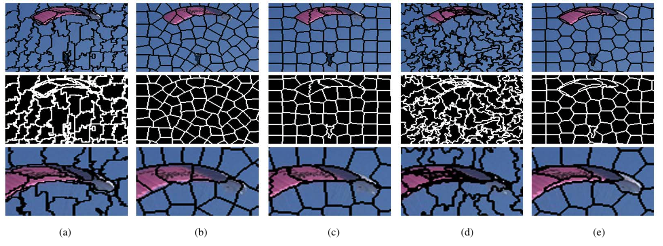
\includegraphics[width = 1 \linewidth]{images/paper2/superpixelsComparison.png}
    \centering
    \caption{Superpixel results from different algorithms. (a) SEEDS. (b) NCuts. (c) SLIC. (d) ERS. (e) LSC.}
    \label{fig: superpixelsComparison}
\end{figure}